\documentclass[oneside,10pt]{memoir}
\usepackage{tutorials}

\usepackage[T1]{fontenc}       % change font encoding to T1
\usepackage[framed,numbered]{matlab-prettifier}

% for visibility of solutions
% \showtrue
\showfalse

% sansserif
%\renewcommand{\familydefault}{\sfdefault}\textbf{}

\newcounter{pass}
\setcounter{pass}{0}


\begin{document}

\tuttitle{Tutorial Questions 02 -- Series}{Dr Killian O'Brien}{6G4Z3006 Calculus}{2025/26 Semester 2}

{\small When possible you should work on the questions in advance and be prepared for discussions on them with your colleagues and tutor. Some questions are straightforward calculation while others require more discussion and thought. The computer icon 
\includegraphics[scale=0.06]{comp.png} indicates where computer calculation or programming may be of use (although it is potentially useful everywhere I guess!).
Further questions can be found in the lecture notes.


\topic{Series notation and defining formulas}
\begin{enumerate}
\item \label{formulas}
Write down some initial terms of the following series
$$\text{(i)} \sum_{n=1}^\infty \frac{(-1)^n}{2n - 1},
\quad \text{(ii)} \sum_{n=1}^\infty \frac{n+1}{n^3 + 2},
\quad \text{(iii)} \sum_{n=1}^\infty \frac{3}{n!},
\quad \text{(iv)} \sum_{n=1}^\infty \left (\sum_{i=1}^n i^{-2} \right ).
$$
\begin{sagesilent}
var('n')
a(n) = (-1)^n/(2*n - 1)
b(n) = (n+1)/(n^3+2)
c(n) = 3/(factorial(n))

A=[a(i) for i in (1..6)]
B=[b(i) for i in (1..6)]
C=[c(i) for i in (1..6)]
D=[sum(1/j^2 for j in range(1,n+1)) for n in (1..6)]
\end{sagesilent}
\begin{solution}
(i) $\sum_{n=1}^\infty \frac{(-1)^n}{2n - 1} = -1 + \frac{1}{3} - \frac{1}{5} + \frac{1}{7} - \frac{1}{9} + \dots$ \\
(ii) $\sum_{n=1}^\infty \frac{n+1}{n^3 + 2} = \frac{2}{3} + \frac{3}{10} + \frac{4}{29} + \frac{5}{66} + \frac{6}{127} + \dots$\\
(iii) $\sum_{n=1}^\infty \frac{3}{n!} = 3 + \frac{3}{2} + \frac{1}{2} + \frac{1}{8} + \frac{1}{40} + \dots $\\
(iv) $ \sum_{n=1}^\infty \left (\sum_{i=1}^n i^{-2} \right )
= \sage{D[0]}+\sage{D[1]}+\sage{D[2]}+\sage{D[3]}+\sage{D[4]}+\sage{D[5]}+\dots$
\end{solution}
\setcounter{pass}{\value{enumi}}
\end{enumerate}
\vskip 2pt
\topic{Series convergence definition}
\begin{enumerate}
\setcounter{enumi}{\value{pass}}
\item
Make sure you can accurately quote the definition of convergence for a series.
\begin{solution}{The series $\sum_{n=1}^\infty a_n$ converges if and only if the associated sequence of partial sums, $\left \{ S_k \right \}_{k=1}^\infty$ where $S_k = \sum_{n=1}^k a_n$, converges. If $S_k \to S$ as $k \to \infty$ then we write $S = \sum_{n=1}^\infty a_n$. Otherwise we say that $\sum_{n=1}^\infty a_n$ diverges.}\end{solution}
\item
Can you confidently give the proof that the harmonic series $\sum_{j=1}^\infty 1/j$ diverges?
\begin{solution}{See notes.}\end{solution}

\item
Can you prove the General Term Test using the definition of convergence?
\begin{solution}{Suppose that $S = \sum_{n=1}^\infty a_n$, i.e. $S_k = \sum_{n=1}^k a_n \to S$ as $k \to \infty$. Note that $a_k = S_k - S_{k-1}$. Let $\epsilon > 0$ be given. By the convergence of the sequence $\{ S_k \}$ there exists a point $K$ such that for all $k \geq K$ we have $|S_k - S| < \frac{\epsilon}{2}$. Then for every $k \geq K+1$ we have
$$|a_k| = |S_k - S_{k-1}| = |S_k - S - (S_{k-1} - S)| \leq |S_k - S| + |S_{k-1} - S| < \frac{\epsilon}{2} + \frac{\epsilon}{2} = \epsilon.$$ This proves the convergence of $a_k$ to 0 as $k \to \infty$.\\
\textit{It's a good idea to use a diagram of the number line here to explain the choice of interval radius $\frac{\epsilon}{2}$ and explain the idea behind this.}}\end{solution}
\setcounter{pass}{\value{enumi}}
\end{enumerate}
\vskip 2pt

\topic{Geometric series test}
\begin{enumerate}
\setcounter{enumi}{\value{pass}}
\item
Ensure that you can derive the partial sum formula for a general geometric series of the form
$$\sum_{n=1}^\infty a r^{n-1}.$$
Can you then prove the convergence/divergence of this series for all possible combinations of values of the initial term $a$ and the common ratio $r$?
\begin{solution}Exploiting the structure of the terms of the geometric series we see that the partial sums $S_k$ satisfy
$$S_k - rS_{k} = a - ar^k$$
which implies that for $r \neq 1$ we have
$$S_k = \frac{a(1-r^k)}{1-r} .$$
Using this we can decide the convergence status of the geometric series.

If $a=0$ then all terms are zero and the series is trivially convergent. So we assume $a \neq 0$ in the following.

If $r=1$ then the series is $\sum_{n=1}^\infty a = a + a + a + \dots $ which is clearly divergent as $a \neq 0$.

If $r=-1$ then the series is $\sum_{n=1}^\infty a(-1)^{n-1} = a - a + a - \dots $ which again is divergent as $a \neq 0$.

In all other cases we can make use of the partial sums formula to say that
$$S = \sum_{n=1}^\infty ar^{n-1} = \lim_{k \to \infty} S_k = \lim_{k \to \infty} \frac{a(1-r^k)}{1-r} .$$
If $|r| > 1$ then the term $r^k$ is divergent and so the series is divergent also. If $|r|<1$ then the term $r^k$ is convergent to 0 and so the series is also convergent and
$$S = \sum_{n=1}^\infty ar^{n-1} = \lim_{k \to \infty} S_k = \lim_{k \to \infty} \frac{a(1-r^k)}{1-r} = \frac{a}{1-r}.$$
\end{solution}
\item
Use the analysis of the ratio test to determine the convergence status and sum if possible, of the series
$$\text{(i)} \, \,  \sum_{n=1}^\infty \frac{2}{3} \left ( \frac{1}{3} \right )^{n+1},
\quad \text{(ii)} \, \, \sum_{n=1}^\infty 3 \left ( \frac{1}{2} \right )^n,
\quad \text{(iii)}\, \,  \sum_{n=1}^\infty \frac{1}{5} \left ( \frac{6}{5} \right )^{n+2}.
$$
\begin{sagesilent}
var('n')
a = sum(2/3 * (1/3)^(n+1),n,1,oo)
b = sum(3 * (1/2)^(n),n,1,oo)
\end{sagesilent}
\begin{solution}
We just need to adjust the term in each case to match the general form of the geometric series used in the previous question and then apply the convergence criteria and formula to get
$$\text{(i)} \, \, \sage{a} , \quad \text{(ii)} \, \, \sage{b} , \quad \text{(iii) divergent}.$$
\end{solution}
\item
Consider the number $a$ with decimal expansion
$$a = 0.1234123412341234 \dots ,$$
continuing in the suggested way. Use the geometric series summation formula to express $a$ as a rational number, i.e. a ratio of integers.
\begin{sagesilent}
var('n')
a = sum(1234/(10000^n),n,1,oo)
\end{sagesilent}
\begin{solution}
We can express $a$ in series form by
$$a = \sum_{n=1}^\infty \frac{1234}{10000^n}.$$
This is a convergent geometric series and applying the sum formula gives
$$a = \sage{a}.$$
\end{solution}
\setcounter{pass}{\value{enumi}}
\end{enumerate}
\vskip 2pt

\topic{Application of the ratio test}
\begin{enumerate}
\setcounter{enumi}{\value{pass}}
\item
Determine the convergence or divergence of the series
$$\sum_{m=0}^\infty \frac{2^m}{m!}.$$
\begin{solution}Writing $a_m$ for the series term the ratio of consecutive terms satisfies
\begin{align*}
\lim_{m \to \infty} \frac{a_{m+1}}{a_m} & = \lim_{m \to \infty} \left ( \frac{2^{m+1}}{(m+1)!} \frac{m!}{2^m} \right ) \\
&= \lim_{m \to \infty} \frac{2}{m+1} \\
& = 0.
\end{align*}
So by the ratio test the series $\sum a_m$ converges.
\end{solution}
\item
Determine the convergence or divergence of the series
$$\sum_{m=0}^\infty \frac{2^m}{(m+1)^2}.$$
\begin{solution}Writing $a_m$ for the series term the ratio of consecutive terms satisfies
\begin{align*}
\lim_{m \to \infty} \frac{a_{m+1}}{a_m} & = \lim_{m \to \infty} \left ( \frac{2^{m+1}}{(m+2)^2} \frac{(m+1)^2}{2^m} \right ) \\
&= \lim_{m \to \infty} 2 \left ( \frac{m+1}{m+2} \right )^2\\
& = 2\lim_{m \to \infty} \left (1 -  \frac{1}{m+2} \right )^2\\
& = 2, \text{ by the algebra of limits theorem for seqs.}
\end{align*}
So by the ratio test the series $\sum a_m$ diverges.
\end{solution}
\item
Does the ratio test give a conclusion about the series
$$\sum_{n=1}^\infty \frac{n}{n+1}?$$
If not, determine the convergence/divergence of this series by more direct means.
\begin{solution}Writing $a_n$ for the series term the ratio of consecutive terms satisfies
\begin{align*}
\lim_{n \to \infty} \frac{a_{n+1}}{a_n} & = \lim_{n \to \infty} \left ( \frac{n+1}{n+2} \frac{n+1}{n} \right ) \\
&= \lim_{n \to \infty} \frac{n^2 + 2n + 1}{n^2 + 2n}\\
&= \lim_{n \to \infty} \frac{1 + 2/n + 1/n^2}{1 + 2/n}\\
& = 1.
\end{align*}
So the ratio test is inconclusive. Looking at the series again we notice that the terms do not converge to zero, in fact
$$\lim_{n \to \infty} a_n = 1.$$
So the series does not pass the General Term Test and so the series is divergent.
\end{solution}
\setcounter{pass}{\value{enumi}}
\end{enumerate}
\topic{Application of comparison tests}
\begin{solution}I tend to prefer the application of the limit comparison test, but anything doable with the limit comparison test can normally be achieved with an equivalent use of the standard comparison test.\end{solution}
\begin{enumerate}
\setcounter{enumi}{\value{pass}}
\item
Use a suitable comparison test to determine the convergence status of the series
$$ \sum_{k=1}^\infty \frac{k^2 + 2}{k(k^2 + 5)}.$$
\begin{solution}The dominant behaviour of the term here is $k^2$ in the numerator and $k^3$ in the denominator so the we should compare to the term $1/k$ which is the term of a divergent series.

Writing $a_k$ for the series term in the question and examining the limit of the ratio we get
\begin{align*}
\lim_{k \to \infty} \frac{a_k}{1/k}
&= \lim_{k \to \infty} \left ( \frac{k^3 + 2k}{k^3 + 5k} \right )\\
&=1
\end{align*}
So the series in question compares with the divergent harmonic series and so by the limit comparison test the series is also divergent.
\end{solution}
\item
Use a suitable comparison test to determine the convergence status of the series
$$ \sum_{k=1}^\infty \frac{k+3}{k(k^2 + 2)}.$$
\begin{solution}The dominant behaviour of the term here is $k^1$ in the numerator and $k^3$ in the denominator so the we should compare to the term $1/k^2$ which is the term of a convergent series.

Writing $a_k$ for the series term in the question and examining the limit of the ratio we get
\begin{align*}
\lim_{k \to \infty} \frac{a_k}{1/k^2}
&= \lim_{k \to \infty} \left ( \frac{k^3 + 3k^2}{k^3 + 2k} \right )\\
&=1
\end{align*}
So the series in question compares with a convergent series and so by the limit comparison test the series is also convergent.
\end{solution}
\setcounter{pass}{\value{enumi}}
\end{enumerate}
\vskip 2pt

\topic{Application of partial fraction expansions}
\begin{sagesilent}
var('n')
a(n) = (9*n^2+33*n+12)/((n+4)*(n+3)*(n+1)*n)
b(n) = 8/(n^2+6*n+5)
c(n) = 9/(n^2+n - 2)
d(n) = (11 - n)/(n^2+6*n+5)
\end{sagesilent}
\begin{enumerate}
\setcounter{enumi}{\value{pass}}
\item
Consider the series $\sum_{n=1}^\infty a_n$ where the term is defined by
$$a_n = \frac{{9 \, n^{2} + 33 \, n + 12}}{{\left(n + 4\right)} {\left(n + 3\right)} {\left(n + 1\right)} n}.$$
Obtain the partial fraction expansion of $a_n$ and use this to obtain the sum of the series.
\begin{solution}{
The partial fraction expansion of $a_n$ is $\sage{a(n).partial_fraction(n)}$ and the sum of the series is $\sage{sum(a(n),n,1,oo)}$.
}\end{solution}
\item
Consider the series $\sum_{n=1}^\infty b_n$ where the term is defined by
$$b_n = \frac{8}{n^2 + 6n + 5}.$$
Obtain the partial fraction expansion of $b_n$ and use this to obtain the sum of the series.
\begin{solution}{
The partial fraction expansion of $b_n$ is $\sage{b(n).partial_fraction(n)}$ and the sum of the series is $\sage{sum(b(n),n,1,oo)}$.
}\end{solution}
\item
Consider the series $\sum_{n=2}^\infty c_n$ where the term is defined by
$$c_n = \frac{9}{n^2 + n - 2}.$$
Obtain the partial fraction expansion of $c_n$ and use this to obtain the sum of the series. (n.b. take note of the starting value of the index $n$)
\begin{solution}{
The partial fraction expansion of $c_n$ is $\sage{c(n).partial_fraction(n)}$ and the sum of the series is $\sage{sum(c(n),n,2,oo)}$.
}\end{solution}
\item
Consider the series $\sum_{n=1}^\infty d_n$ where the term is defined by
$$d_n = \frac{11 - n}{n^2 + 6n +5}.$$
Obtain the partial fraction expansion of $d_n$ and use this to decide whether the series is convergent or divergent.
\begin{solution}{
The partial fraction expansion of $d_n$ is $\sage{d(n).partial_fraction(n)}$. Because the numerators are different we do not get complete cancellation. Considering the partial sum $S_k$ we see that
$$S_k = \frac{3}{2}+\frac{3}{3} + \frac{3}{4} + \frac{3}{5}  - \left (\sum_{n=6}^{k+1} \frac{1}{n} \right ) -\frac{4}{k+2} - \frac{4}{k+3} - \frac{4}{k+4} - \frac{4}{k+5}.$$
We see that $S_k$ contains, essentially, the partial sum of the harmonic series. Since the harmonic series diverges then so does the sequence $S_k$ and hence the series in question is divergent.

Alternatively we can apply the limit comparison test to this series, comparing with the harmonic series, and this will also show that it is divergent.}\end{solution}
\setcounter{pass}{\value{enumi}}
\end{enumerate}
\vskip 2pt

\topic{Computer work} \comp
\begin{enumerate}
\setcounter{enumi}{\value{pass}}
\item
You should ensure that you are able to use Matlab to build an array containing a specified number of initial terms of a series.
\item
\label{q:matlab}
You should then be able to build an array containing the partial sums of that series and plot them as visual aid to determining the long term behaviour of the series.

\begin{solution}
The following Matlab code constructs and plots the first 100 partial sums of the series $\sum_{n=1}^\infty 1/n^2$.

\end{solution}
\begin{lstlisting}[
  style      = Matlab-editor,
  basicstyle = \mlttfamily,
]
x = @(n) 1/n^2 % creates a function handle x for the series term
N = [1:100] % the index values 1, 2, 3, ..., 100
Xseries = arrayfun(x,N) % a vector of values 1/n^2
Xpartials = cumsum(Xseries) % the cumsum function creates a vector of cumulative (partial) sums
plot(Xpartials,'.') % plots the partial sums
\end{lstlisting}
\begin{center}
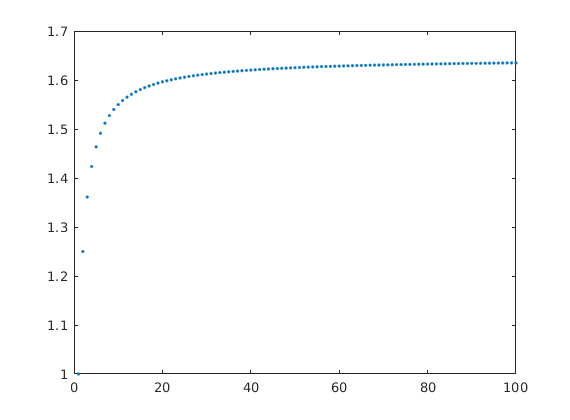
\includegraphics[scale=0.7]{series.png}
\end{center}



\item
Investigate the capabilities of Matlab's \texttt{symsum} command from its symbolic toolbox. See the information at \url{http://uk.mathworks.com/help/symbolic/symsum.html}.
\item
Apply these techniques to the series mentioned in this problem sheet, the questions in the lecture notes, etc
\item
Investigate the capabilities of other computer systems, such as SageMath in this regard. Register for a free account at \url{https://cocalc.com} and check out Gregory Bard's book \emph{Sage for Undergraduates} available from \url{http://www.gregorybard.com/Sage.html}.

\begin{solution}
For example. Here is some SageMath code for plotting the $1/n^2$ series shown in question \ref{q:matlab}
\end{solution}
\begin{lstlisting}[
  style      = Matlab-editor,
  basicstyle = \mlttfamily,
]
Xseries = [1/n^2 for n in range(1,101)]
Xpartials = [sum(Xseries[:k]) for k in range(1,100)]
list_plot(Xpartials)
\end{lstlisting}
\begin{center}
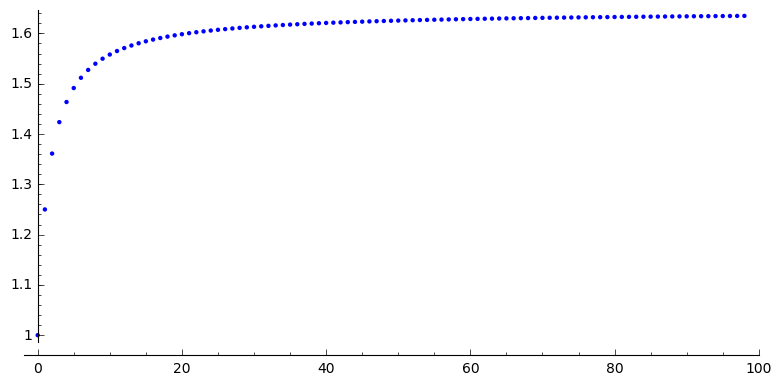
\includegraphics[scale=0.7]{sageseries.png}
\end{center}
\setcounter{pass}{\value{enumi}}
\end{enumerate}
\vskip 2pt

\topic{Further problems}
{\small In these problems there is not so much guidance given about which particular convergence test to use. Sometimes it is a process of trial and error but with experience and understanding of the different tests one can often identify the appropriate test from the form of the given series.}
\begin{enumerate}
\setcounter{enumi}{\value{pass}}
\item
Investigate and prove the convergence/divergence of the following series.
$$\text{(i) } \sum_{n=1}^\infty \frac{n^3}{n^5 + 2}
\quad \quad \text{(ii) } \sum_{n=1}^\infty \frac{3^n}{5^n + 5}
\quad \quad \text{(iii) } \sum_{n=1}^\infty \frac{n}{3^n} .$$

\begin{solution}
(i) Perform a comparison test with the convergent series $\sum 1/n^2$ to conclude that the given series is convergent. For the standard comparison test we have
$$\frac{n^3}{n^5 + 2} < \frac{n^3}{n^5} = \frac{1}{n^2}.$$
For the limit comparison test we have
$$\lim_{m \to \infty} \left ( \frac{n^3}{n^5 + 2}  \frac{1}{1/n^2} \right ) = \lim_{m \to \infty} \frac{n^5}{n^5 +2} = \lim_{m \to \infty} \frac{1}{1 + 2/n^5} = \frac{1}{1+0} = 1.$$

(ii) Perform a comparison test with the convergent geometric series $\sum_{n=1}^\infty \frac{3}{5} (\frac{3}{5})^{n-1}$ to conclude that the given series is convergent. The inequality is
$$\frac{3^n}{5^n + 5} < \frac{3^n}{5^n} = \frac{3}{5}\left ( \frac{3}{5} \right )^{n-1}.$$

(iii)
Perform the ratio test. The limit of the ratio of consecutive terms is
$$\lim_{n \to \infty} \frac{n+1}{3^{n+1}} \frac{3^n}{n} = \lim_{n \to \infty} \frac{n+1}{3n} = \lim_{n \to \infty} \frac{1+1/n}{3} = \frac{1}{3}.$$
As $ 0 \leq \frac{1}{3} < 1$ the given series is convergent.
\end{solution}

\item
The series $\sum_{n=1}^\infty n^a / (2+n^3)$ depends on the value of the parameter $a$. For which values of $a$ will the series converge? For which values of $a$ will it diverge?

\begin{solution}
These series call for an application of the limit comparison test. As the comparison series we will use the hyper-harmonic series $\sum 1/n^{a-3}$. Applying the limit comparison test we get
$$\lim \left ( \frac{n^a}{2+n^3} \frac{1}{1/n^{a-3}} \right ) = \lim \left ( \frac{n^a}{2+n^3} n^{3-a} \right ) = \lim \frac{n^3}{2+n^3} = \lim \frac{1}{2/n^3 + 1} = \lim \frac{1}{0+1} = 1.$$
The conclusion is that the given series has the same convergent/divergent behaviour as the series $\sum 1/n^{a-3}$. This comparison series is convergent for $a > 4$ and divergent for $a \leq 4$ (by the result about hyper-harmonic series obtained from the integral test.)
\end{solution}



\item
Investigate and prove the convergence or divergence of the series
$$\sum_{n=1}^\infty \frac{n! (n+1)!}{(3n)!}.$$
\begin{solution}
The ratio test can be applied to this series and you should find that it is a convergent series.
\end{solution}

\item
Investigate and prove the convergence or divergence of the series
$$\sum_{n=1}^\infty (-1)^n \cos \left ( \frac{1}{n} \right ).$$
\begin{solution}
This is an alternating series but the absolute value of the terms, $\cos(1/n)$, is converging to 1. So the series is not convergent, by the alternating series test.
\end{solution}

\item
Consider the power series
$$\sum_{n=0}^\infty \frac{n^3}{n^4 +1} x^{3n}.$$
What is the radius of convergence of this power series?
\begin{solution}
The radius of convergence is obtained from applying the ratio test to the power series terms. The power series will converge if $x$ satisfies
\begin{align*}
&\lim_{n \to \infty} \left | \frac{(n+1)^3}{(n+1)^4 +1} x^{3(n+1)} \frac{n^4+1}{n^3} x^{-3n} \right |
 < 1\\
 \Leftrightarrow &\lim_{n \to \infty} \left | \frac{(n+1)^3(n^4+1)}{((n+1)^4 +1)n^3} x^{3} \right |
 < 1\\
 \Leftrightarrow & |x^3|<1, \text{ applying algebra of limits theorem to ratio of polynomials} \\
 \Leftrightarrow & |x| < 1.
\end{align*}
So the radius of convergence of this power series is 1.
\end{solution}

\item \label{q:twogeometric}
Can you find the precise value of the series
$$\sum_{n=1}^\infty \frac{1+2^n}{3^{n-1}}?$$
\textit{Hint: Which series convergence test(s) allow you to find the actual values of infinite sums?}
\begin{solution}
We can split that partial sums of this series into the sum of the partial sums of two convergent geometric series, i.e.
$$\sum_{n=1}^k \frac{1+2^n}{3^{n-1}} = \left ( \sum_{n=1}^k \left ( \frac{1}{3} \right )^{n-1} \right )+ 2\sum_{n=1}^k \left ( \frac{2}{3} \right )^{n-1} . $$
We can then apply the algebra of limits theorem for sequences and the Geometric Series formula to get the sum of the given series.
\end{solution}

\item
Does the series $\sum_{n=1}^\infty \frac{n+5}{n\sqrt{n+3}}$ converge?
\begin{solution}
This series is divergent as it compares to $\sum 1/n^{1/2}$, which is a divergent hyper-harmonic series. Use a standard or limit comparison test to prove the divergence.
\end{solution}

\item
Does the series $\sum_{n=1}^\infty \frac{3+\cos(n)}{e^n}$ converge?
\begin{solution}
This series converges as it compares to a convergent geometric series with common ratio $1/e$. Use a standard comparison test to prove the convergence, using the inequality
$$ 0 < \frac{3+\cos(n)}{e^n} \leq \frac{4}{e^n} = \frac{4}{e} \left ( \frac{1}{e} \right )^{n-1}.$$
\end{solution}


\item
Does the series $\sum_{n=0}^\infty (-1)^n (n^2+1)^{-1/2}$ converge? Does it converge absolutely?
\textit{Hint: The presence of the $(-1)^n$ terms means we should apply the \rule{\widthof{alternating series}}{0.5pt} test}
\begin{solution}
This is a convergent series. Prove this by applying the alternating series test.
\end{solution}

\item
What is the value of the sum
$$\sum_{n=1}^\infty \frac{2^n + 5^n}{7^n}?$$
\begin{solution}
Like question \ref{q:twogeometric}, the partial sums of this series can be expressed as the sum of the partial sums from two convergent geometric series. So we can obtain the sum of the given series by applying the algebra of limits theorem for the sequences of partial sums together with the Geometric Series formula.
\end{solution}

\item
Will the series
$$\sum_{n=1}^\infty (-1)^n \frac{n}{1+n^2}$$
converge? Will it converge absolutely?
\begin{solution}
The given series is convergent by the alternating series test. But it does not converge absolutely as the series of absolute values, $\sum n/(1+n^2)$, compares to the divergent harmonic series $\sum 1/n$.
\end{solution}


\end{enumerate}

\end{document}


